\section{Modelli di Ciclo di Vita}

\begin{definition}[Processo Software]
    Con processo software si indica il percorso da seguire per sviluppare un prodotto o più nello specifico un software.
    Fanno parte del processo sia gli strumenti e le tecniche per lo sviluppo che i professionisti coinvolti.
\end{definition}

\subsection{Modelli Sequenziali}

\subsubsection{Build-and-Fix}

Il prodotto è sviluppato senza alcuna fase di progettazione preliminare, lo sviluppatore scrive il software
e poi lo modifica ogni volta che non soffisfa il committente.

\paragraph{\textcolor{red}{Contro}}

Diventa improponibile per progetti grandi e la manutenzione diventa difficile senza documentazione nè specifica.

\subsubsection{Modello a Cascata}

Questo modello è stato il primo a distingure il processo software in più fasi, evidenziando l'importanza della progettazione e dell'analisi.

Viene chiamato anche modello \emph{\textcolor{cyan}{document driven}} dato che ogni fase produce un documento, e per passare alla successiva
occorre aver approvato il documento della fase precedente.

\paragraph{\textcolor{red}{Contro}} Troppo pesante da seguire, inoltre non si può tornare indietro, e mancando
l'interazione con il cliente, se non è soddisfatto, và tutto ripetuto dall'inizio.

\subsubsection{Modello a V}

\begin{center}
    \begin{figure}[h]
            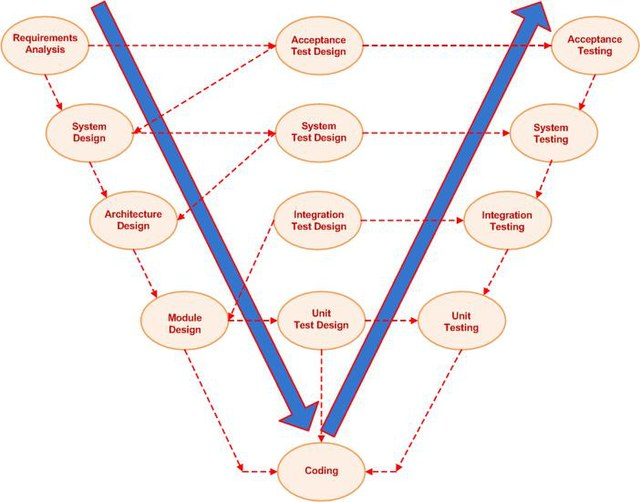
\includegraphics[scale=0.5]{img/V-model.JPG}
        \caption{Le frecce blu rappresentano il \emph{tempo}, mentre quelle tratteggiate le \emph{dipendenze}}
    \end{figure}
\end{center}

Questo modello evidenzia come sia possibile progettare i \textcolor{cyan}{test}
durante le fasi di sviluppo (quelle a sinistra, prima della fase di \emph{coding}). Mentre sulla destra
sono presenti i test veri e propri che devono verificare e convalidare l'attività in corrispondenza sulla sinistra.

\paragraph{\textcolor{ForestGreen}{Standard SQA}}
Questo modello è uno degli standard \emph{SQA} (Software Quality Assurance), usato
per descrivere le attività di test durante il processo di sviluppo.

\subsection{Modelli Iterativi}

\subsubsection{Rapid Prototyping}

L'obbiettivo è quello di costruire rapidamente un prototipo del software per permettere al committente di sperimentarlo.

Questo modello diventa utile quando i requisiti non sono chiari, quindi ogni prototipo aiuterà il cliente a descriverli meglio.

\begin{center}
    \begin{tikzpicture}[main/.style={rectangle, draw}]
        \node[main] (1) {Analisi Preliminare};
        \node[main] (2) [below right=1cm and 0.1cm of 1] {Analisi e Progettazione};
        \node[main] (3) [below right=1cm and 0.1cm of 2] {\begin{tabular}{c}Realizzazione del \\ prototipo (usa e getta)\end{tabular}};
        \draw[thick, ->] (1) -| (2);
        \draw[thick, ->] (2) -| (3);
        \draw[thick, ->] (3) -| (2);
    \end{tikzpicture}
\end{center}

\subsubsection{Modello Incrementale}

Il software viene costruito in modo iterativo, aggiungendo di volta in volta nuove funzionalità.

I requisiti e la progettazione vengono definiti inizialmente, per questo è possibile applicarlo solo in caso di requisiti stabili.

\paragraph{\textcolor{red}{Contro}}
Se non viene realizzata una buona progettazione, questo modello sfocia in un \emph{Build-and-Fix}.

\begin{center}
    \begin{tikzpicture}[main/.style={rectangle, draw}]
        \node[main] (1) {Analisi e Progettazione};
        \node[main] (2) [below right=0.5cm and -2cm of 1] {\begin{tabular}{c} Progettazione di dettaglio \\ (implemento una singola funzionalità) \end{tabular}};
        \node[main] (3) [below right=1cm and -1.5cm of 2] {\begin{tabular}{c} Realizzazione versione \\ incompleta \end{tabular}};
        \draw[thick, ->] (1) -| (2);
        \draw[thick, ->] (2) -| (3);
        \draw[thick, ->] (3) -| (2);
    \end{tikzpicture}
\end{center}

\newpage

\subsubsection{Modello a Spirale}

In questo caso ogni iterazione è formata da 4 fasi che corrispondono ai quadranti del piano:
\begin{enumerate}
    \item \emph{Quadrante in alto a sinistra}: definizione degli obiettivi e dei vincoli.
    \item \emph{Quadrante in alto a destra}: analisi e risoluzione dei rischi.
    \item \emph{Quadrante in basso a destra}: sviluppo e verifica del prossimo livello.
    \item \emph{Quadrante in basso a sinistra}: pianificazione della fase successiva.
\end{enumerate}

Questo modello viene anche chiamato \emph{\textcolor{cyan}{risk driven}} in quanto è incentrato principalmente sull'analisi
dei rischi. Inoltre si ispira profondamente al metodo iterazivo \emph{\textcolor{cyan}{plan-do-check-act cycle}} \footnote{\url{https://it.wikipedia.org/wiki/Ciclo_di_Deming}}

\begin{figure}[h]
    \begin{center}
        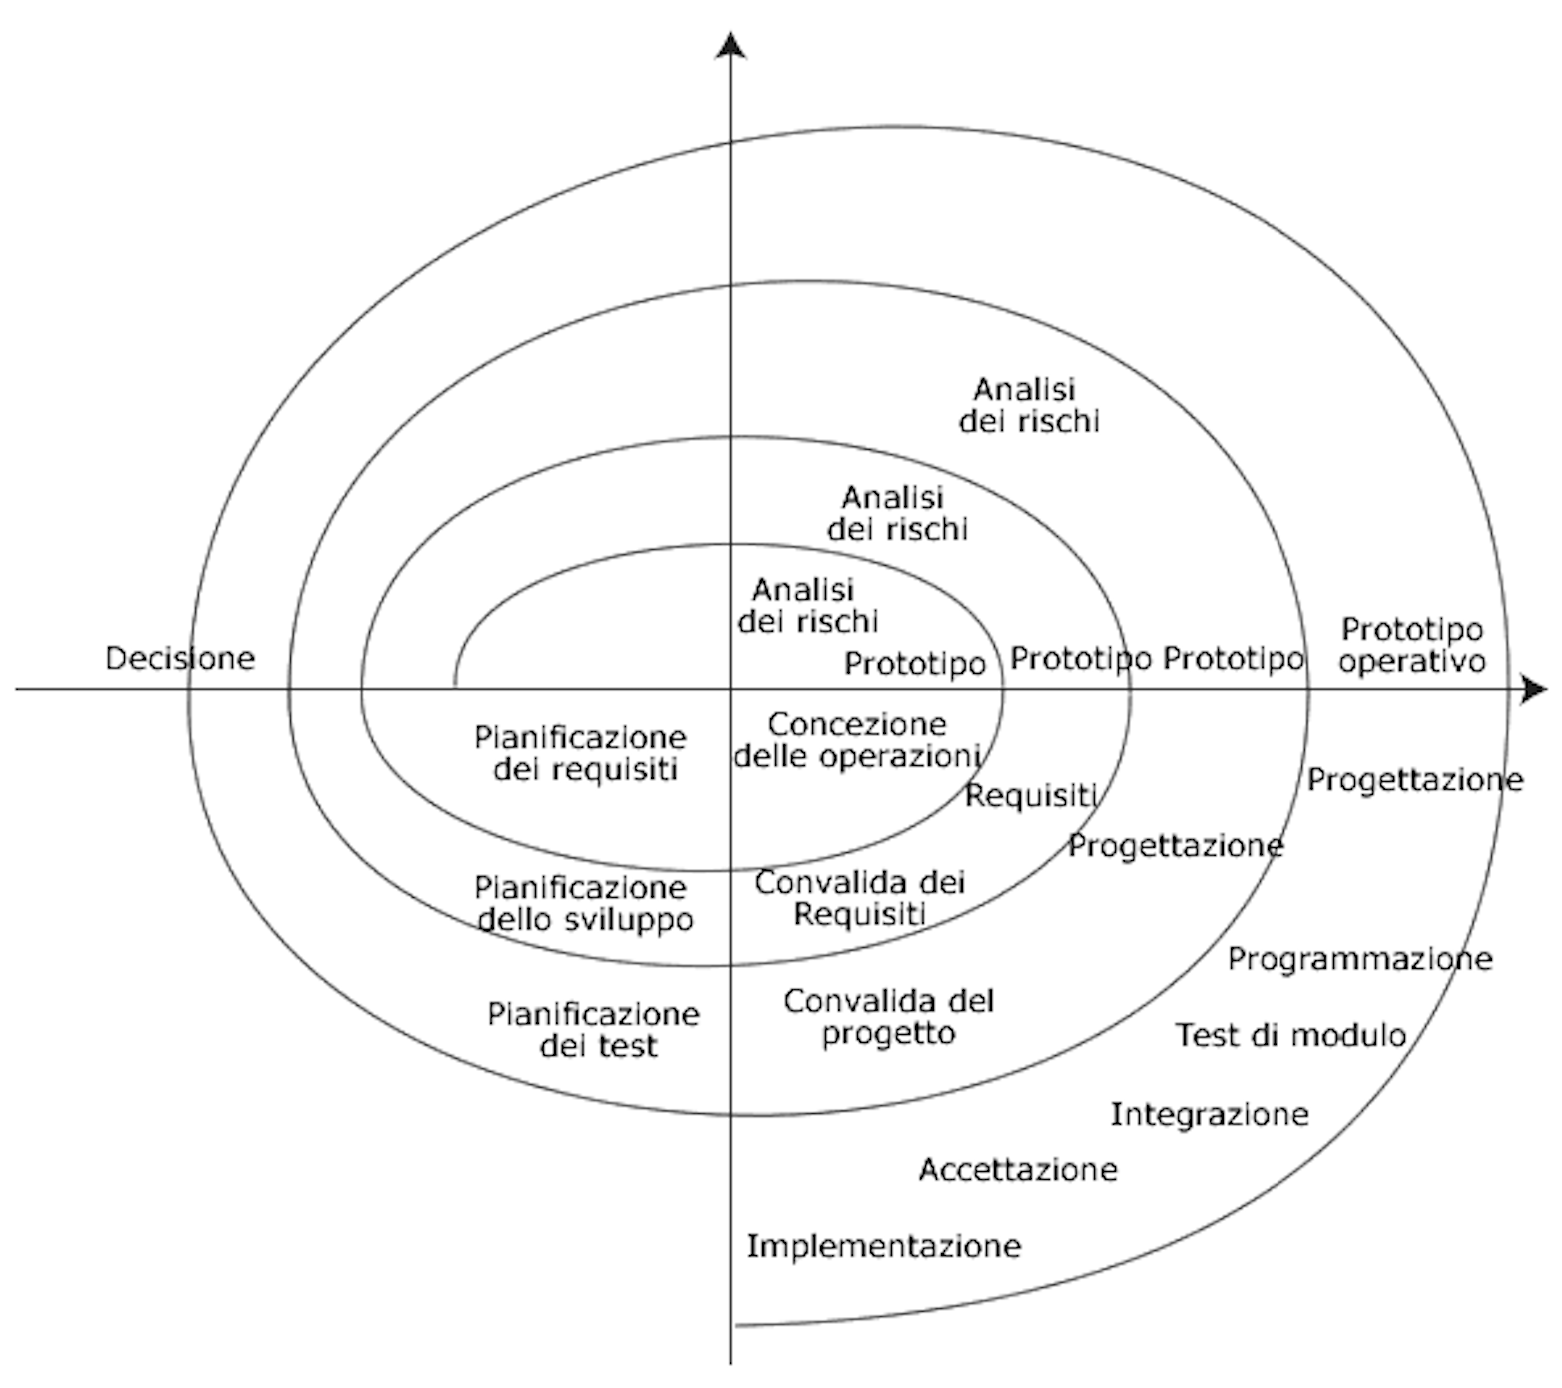
\includegraphics[scale=0.4]{img/modellospirale.png}
    \end{center}
\end{figure}

\subsection{Unified Process}

In questo modello vengono distinte quattro fasi chiamate \emph{\textcolor{cyan}{Inception}}, \emph{\textcolor{cyan}{Elaboration}}, \emph{\textcolor{cyan}{Construction}}
e \emph{\textcolor{cyan}{Transition}}. Ogni fase può presentare un numero variabile di iterazioni anche in base alla dimensione
del progetto.

Questo modello viene definito \textcolor{cyan}{iterativo incrementale}, \emph{incrementale} perchè
alla fine di ogni iterazione si ottiene un rilascio del sistema con funzionalità in più o migliorate
rispetto al rilascio precedente.

Inoltre viene data molta importanza all'architettura del sistema, infatti già dalle prime fasi ci si
concentra soprattutto sull'architettura anche se a livello molto superficiale, lasciando i dettagli alle fasi successive. In questo
modo è molto facile avere una visione generale del sistema che sarà facilmente modellabile sulla variazione dei requisiti. Per
questo, piuttosto che dai requisiti, ci si fà guidare principalmente dai \emph{casi d'uso} e dall'\emph{analisi dei rischi}.

\begin{figure}[h]
    \begin{center}
        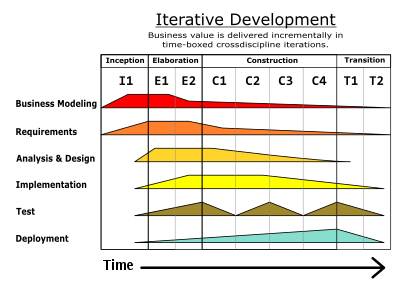
\includegraphics[scale=0.8]{img/unified_process.png}
    \end{center}
\end{figure}

\subsection{Processi Agili}

\begin{definition}[Metodo Agile]
    Con \textcolor{cyan}{metodo agile} si intende un metodo per lo sviluppo del software
    che si basa principalmente sul coinvolgimento del committente.
    Questa metodologia si riferisce ai principi del \emph{\textcolor{cyan}{Manifesto di Snowbird}} del 2001.
\end{definition}

I concetti chiave di questi processi sono:

\begin{itemize}
    \item \textcolor{cyan}{Continuous Integration}: rendere il più automatico possibile la consegna e l'integrazione dei singoli moduli.
    \item \textcolor{cyan}{Continuous Delivery}: rilascio frequente e supportato delle nuovi versioni del software.
    \item \textcolor{cyan}{DevOps}: \emph{Development} e \emph{Operations}, ovvero maggiore collaborazione tra sviluppatori e responsabili della
        manutenzione, della sicurezza e dell'infrastruttura dell'azienda.
\end{itemize}

\subsubsection{Il Manifesto di Snowbird}

Il \emph{Manifesto di Snowbird} si fonda su quattro punti fondamentali:

\begin{enumerate}
    \item \textcolor{cyan}{Comunicazione}: la comunicazione fra tutti gli attori del progetto è centrale, soprattutto le interazioni e
        la collaborazione con i clienti.
    \item \textcolor{cyan}{Semplicità}: si mantiene il codice sorgente il più semplice possibile, ma comunque avanzato tecnicamente,
        in questo modo si riduce la documentazione al minimo indispensabile.
    \item \textcolor{cyan}{Feedback}: sin dal primo giorno di sviluppo il codice viene testato, in modo da poter rilasciare versioni ad intervalli molto frequenti.
    \item \textcolor{cyan}{Coraggio}: dare in uso il sistema il prima possibile ed implementare i cambiamenti richiesti man mano.
\end{enumerate}

Di seguito sono riportati due modelli che si basano sui \emph{processi agili}.

\subsubsection{eXtreme Programming}

Si basa su un insieme di consuetudini:

\begin{itemize}
    \item \emph{Pianificazione flessibile}: è basata su un insieme di scenari proposti dagli utenti e i programmatori vengono coinvolti direttamente.
    \item \emph{Rilasci frequenti}: più o meno ogni 2-4 settimane, e alla fine si ricomincia con una nuova pianificazione.
    \item \emph{Progetti semplici}: comprensibili a tutti.
    \item \emph{Testing}: test basati sui singoli scenari e con supporto automatico.
    \item \emph{Test Driven Development}: i casi di test vengono definiti prima della scrittura del codice.
    \item \emph{Cliente sempre a disposizione}
    \item \emph{Programmazione a coppie}: viene usato un solo terminale, una persona svolge il ruolo di \emph{\textcolor{cyan}{driver}}
        che scrive il codice, mentre un'altra fà il \emph{\textcolor{cyan}{navigatore}}, ovvero controlla il lavoro del \emph{driver} attivamente.
    \item \emph{No al lavoro straordinario}
    \item \emph{Collettivizzazione del codice}: accesso libero e continua integrazione.
    \item \emph{Code Refactoring}: modificare il codice senza cambiare il suo comportamento e commentarlo il più possibile.
    \item \emph{Daily Stand Up Meeting}
\end{itemize}

\subsubsection{SCRUM}

\begin{definition}[SCRUM]
    Con \emph{\textcolor{cyan}{SCRUM}} si intende un processo \emph{iterativo} ed \emph{incrementale}, dove alla fine
    di ogni iterazione vengono rilasciate un insieme di funzionalità potenzialmente rilasciabili.
\end{definition}

Il processo è diviso in tre fasi:

\begin{enumerate}
    \item \textbf{\textcolor{cyan}{Pre-game phase}}: 
        \begin{enumerate}
            \item \textcolor{cyan}{Planning sub-phase}: viene creata una \emph{\textcolor{cyan}{Product Backlog List}}
                che contiene tutti i requisiti conosciuti.
            \item \textcolor{cyan}{Architecture sub-phase}: viene già pianificato il design di alto livello e l'architettura del sistema.
        \end{enumerate}
    \item \textbf{\textcolor{cyan}{Development phase}}: in questa fase il sistema viene sviluppato attraverso una serie di \emph{\textcolor{cyan}{Sprint}},
        ovvero cicli iterativi nei quali vengono sviluppate o migliorate una serie di funzionalità, e ogni sprint può durare circa 1-4 settimane. Lo \emph{Sprint} ovviamente
        include le classiche fasi di sviluppo del software.
    \item \textbf{\textcolor{cyan}{Post-game phase}}: il prodotto viene preparato per il rilascio, ovvero si prepara l'\emph{integrazione},
        i \emph{test}, la \emph{documentazione} per l'utente e la preparazione del materiale di \emph{marketing}.
\end{enumerate}

I ruoli principali durante l'esecuzione di un processo \emph{SCRUM} sono tre:

\begin{itemize}
    \item \textbf{\textcolor{cyan}{Product Owner}}: ci si riferisce a quella persona responsabile di accettare o rifiutare i risultati di un lavoro e di poter terminare uno \emph{Sprint}, inoltre
        fà da raccordo fra tutti soggetti interessati nel progetto.
    \item \textbf{\textcolor{cyan}{Membri del Team}}: i membri decidono cosa fare in ogni \emph{Sprint}, ogni team è indipendente e i membri non fanno capo ad alcun project manager.
        Ogni membro ha diverse specializzazioni (\emph{cross-functional}), in modo tale da non avere persone con troppo carico di lavoro e ognuno si occupa di un singolo lavoro alla volta.
    \item \textbf{\textcolor{cyan}{Scrum Master}}: non ha alcuna autorità sul team, ma si occupa di supportarlo e motivarlo, garantendo anche le condizioni ambientali per lavorare al meglio.
\end{itemize}

\paragraph{Kanban Board} Questa lavagna permette di gestire al meglio il flusso del lavoro. Come mostrato in figura è presente
un \emph{\textcolor{cyan}{Work In Progress Limit}} che definisce un limite alla quantità di post-it che possono essere presenti in
ogni colonna. Questo limite permette di completare più velocemente i singoli lavori, in modo tale di dare qualcosa al cliente il prima possibile e di
individuare facilmente i \textcolor{cyan}{colli di bottiglia} che possono rallentare gli altri lavori.
Inoltre permette di ridurre il \emph{\textcolor{cyan}{task switching}}, ovvero il lavoro su più task contemporaneamente.

\begin{figure}[h]
    \begin{center}
        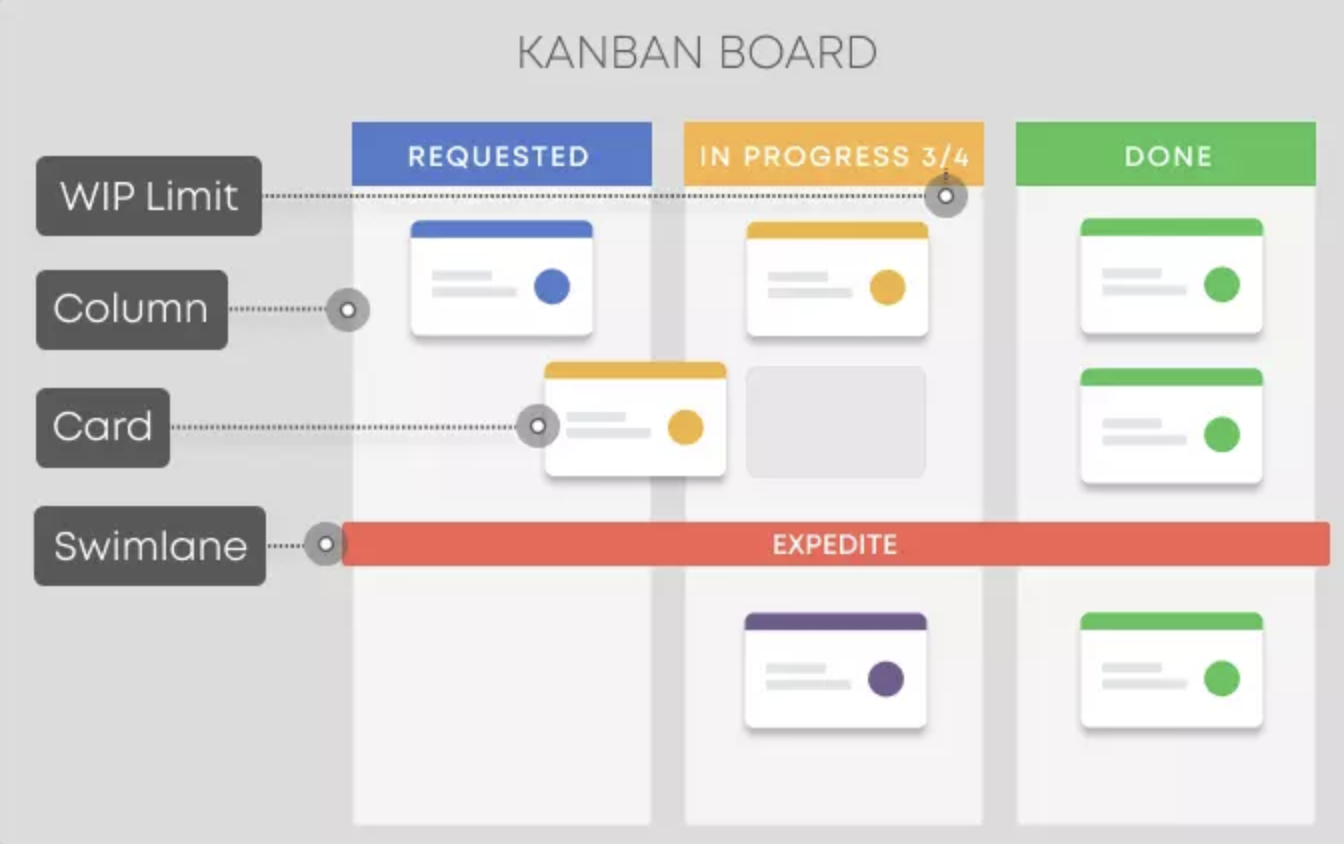
\includegraphics[scale=0.5]{img/kanboard.png}
    \end{center}
\end{figure}

Gli eventi che fanno parte di uno \emph{Sprint} sono i seguenti:
\begin{enumerate}
    \item \textcolor{cyan}{Sprint planning}: il \emph{product owner} gestisce l'evento di pianificazione dello \emph{Sprint}.
    \item \textcolor{cyan}{Daily meeting}: i membri del team e gli SCRUM master si ritrovano davanti la \emph{kanban} e discutono delle
        difficultà che hanno riscontrato.
    \item \textcolor{cyan}{Review}: alla fine di di una modifica concreta al software, questo viene ispezionato in collaborazione con gli utenti per ottenere un feedback
        e per discutere su cambiamenti o nuove idee.
    \item \textcolor{cyan}{Retrospettiva}: questa fase permette di riflettere, studiare e adattarsi per lo \emph{Sprint} successivo.
\end{enumerate}